%package list
\documentclass{article}
\usepackage[top=3cm, bottom=3cm, outer=3cm, inner=3cm]{geometry}
\usepackage{multicol}
\usepackage{graphicx}
\usepackage{url}
%\usepackage{cite}
\usepackage{hyperref}
\usepackage{array}
%\usepackage{multicol}
\newcolumntype{x}[1]{>{\centering\arraybackslash\hspace{0pt}}p{#1}}
\usepackage{natbib}
\usepackage{pdfpages}
\usepackage{multirow}
\usepackage[normalem]{ulem}
\useunder{\uline}{\ul}{}
\usepackage{svg}
\usepackage{xcolor}
\usepackage{listings}
\lstdefinestyle{ascii-tree}{
    literate={├}{|}1 {─}{--}1 {└}{+}1 
  }
\lstset{basicstyle=\ttfamily,
  showstringspaces=false,
  commentstyle=\color{red},
  keywordstyle=\color{blue}
}
%\usepackage{booktabs}
\usepackage{caption}
\usepackage{subcaption}
\usepackage{float}
\usepackage{array}

\newcolumntype{M}[1]{>{\centering\arraybackslash}m{#1}}
\newcolumntype{N}{@{}m{0pt}@{}}


%%%%%%%%%%%%%%%%%%%%%%%%%%%%%%%%%%%%%%%%%%%%%%%%%%%%%%%%%%%%%%%%%%%%%%%%%%%%
%%%%%%%%%%%%%%%%%%%%%%%%%%%%%%%%%%%%%%%%%%%%%%%%%%%%%%%%%%%%%%%%%%%%%%%%%%%%
\newcommand{\itemEmail}{}
\newcommand{\itemStudent}{Jose Gabriel Quispe Mamani}
\newcommand{\itemCourse}{Programación Web 1}
\newcommand{\itemCourseCode}{20233633}
\newcommand{\itemSemester}{I}
\newcommand{\itemUniversity}{Universidad Nacional de San Agustín de Arequipa}
\newcommand{\itemFaculty}{Facultad de Ingeniería de Producción y Servicios}
\newcommand{\itemDepartment}{Departamento Académico de Ingeniería de Sistemas e Informática}
\newcommand{\itemSchool}{Escuela Profesional de Ingeniería de Sistemas}
\newcommand{\itemAcademic}{2024 - B}
\newcommand{\itemInput}{Del 15 Octubre 2024}
\newcommand{\itemOutput}{Al 27 Octubre 2024}
\newcommand{\itemPracticeNumber}{05}
\newcommand{\itemTheme}{Expresiones Regulares}
%%%%%%%%%%%%%%%%%%%%%%%%%%%%%%%%%%%%%%%%%%%%%%%%%%%%%%%%%%%%%%%%%%%%%%%%%%%%
%%%%%%%%%%%%%%%%%%%%%%%%%%%%%%%%%%%%%%%%%%%%%%%%%%%%%%%%%%%%%%%%%%%%%%%%%%%%

\usepackage[english,spanish]{babel}
\usepackage[utf8]{inputenc}
\AtBeginDocument{\selectlanguage{spanish}}
\renewcommand{\figurename}{Figura}
\renewcommand{\refname}{Referencias}
\renewcommand{\tablename}{Tabla} %esto no funciona cuando se usa babel
\AtBeginDocument{%
	\renewcommand\tablename{Tabla}
}

\usepackage{fancyhdr}
\pagestyle{fancy}
\fancyhf{}
\setlength{\headheight}{30pt}
\renewcommand{\headrulewidth}{1pt}
\renewcommand{\footrulewidth}{1pt}
\fancyhead[L]{\raisebox{-0.2\height}{
\includegraphics[width=3cm]{img/logo_episunsa.png}}}
\fancyhead[C]{\fontsize{7}{7}\selectfont	\itemUniversity \\ \itemFaculty \\ \itemDepartment \\ \itemSchool \\ \textbf{\itemCourse}}
\fancyhead[R]{\raisebox{-0.2\height}{
\includegraphics[width=1.2cm]{img/logo_abet}}}
\fancyfoot[L]{Estudiante Jose G.Quispe Mamani}
\fancyfoot[C]{\itemCourse}
\fancyfoot[R]{Página \thepage}

% para el codigo fuente
\usepackage{listings}
\usepackage{color, colortbl}
\definecolor{dkgreen}{rgb}{0,0.6,0}
\definecolor{gray}{rgb}{0.5,0.5,0.5}
\definecolor{mauve}{rgb}{0.58,0,0.82}
\definecolor{codebackground}{rgb}{0.95, 0.95, 0.92}
\definecolor{tablebackground}{rgb}{0.8, 0, 0}

\lstset{frame=tb,
	language=bash,
	aboveskip=3mm,
	belowskip=3mm,
	showstringspaces=false,
	columns=flexible,
	basicstyle={\small\ttfamily},
	numbers=none,
	numberstyle=\tiny\color{gray},
	keywordstyle=\color{blue},
	commentstyle=\color{dkgreen},
	stringstyle=\color{mauve},
	breaklines=true,
	breakatwhitespace=true,
	tabsize=3,
	backgroundcolor= \color{codebackground},
}

\begin{document}
	
	\vspace*{10px}
	
	\begin{center}	
		\fontsize{17}{17} \textbf{ Informe de Laboratorio \ 05}
	\end{center}
	\centerline{\textbf{\Large Tema: \itemTheme}}
	%\vspace*{0.5cm}	

	\begin{flushright}
		\begin{tabular}{|M{2.5cm}|N|}
			\hline 
			\rowcolor{tablebackground}
			\color{white} \textbf{Nota}  \\
			\hline 
			     \\[30pt]
			\hline 			
		\end{tabular}
	\end{flushright}	

	\begin{table}[H]
		\begin{tabular}{|x{4.7cm}|x{4.8cm}|x{4.8cm}|}
			\hline 
			\rowcolor{tablebackground}
			\color{white} \textbf{Estudiante} & \color{white}\textbf{Escuela}  & \color{white}\textbf{Asignatura}   \\
			\hline 
			{\itemStudent \par \itemEmail} & \itemSchool & {\itemCourse  \par \par Código:\itemCourseCode}     \\
			\hline 			
		\end{tabular}
	\end{table}		
	
	\begin{table}[H]
		\begin{tabular}{|x{4.7cm}|x{4.8cm}|x{4.8cm}|}
			\hline 
			\rowcolor{tablebackground}
			\color{white}\textbf{Laboratorio} & \color{white}\textbf{Tema}  & \color{white}\textbf{Duración}   \\
			\hline 
			\itemPracticeNumber & \itemTheme & 04 horas   \\
			\hline 
		\end{tabular}
	\end{table}
	
	\begin{table}[H]
		\begin{tabular}{|x{4.7cm}|x{4.8cm}|x{4.8cm}|}
			\hline 
			\rowcolor{tablebackground}
			\color{white}\textbf{Semestre académico} & \color{white}\textbf{Fecha de inicio}  & \color{white}\textbf{Fecha de entrega}   \\
			\hline 
            \itemAcademic & \itemInput &  \itemOutput \\
			\hline 
		\end{tabular}
	\end{table}
	
	\section{Tarea}
En esta tarea usted deberá implementar un pequeño sistema web que simule            una calculadora que permita realizar las operaciones aritméticas básicas (suma, resta, multiplicación y división). 
        \subsection{Restricciones}
	\begin{itemize}		
		\item No deberá consultar sitios web ajenos a los dados en el curso.
		\item Deberán hacer dos directorios: css, cgi-bin.
		\item Deberán trabajar con formularios, el cual deberá tener un único botón "calcular".
  \item Usar expresiones regulares para reconocer los 2 operandos y el operador.  Además puntos extra si en la expresión se reconoce paréntesis.
  \item Indentar correctamente su código.

	\end{itemize}
		
	\section{Equipos, materiales y temas utilizados}
	\begin{itemize}
		\item Sistema Operativo Ubuntu 24.04 LTS.
		\item Docker version 27.3.1.
		\item Perl 5.38.0.
		\item Expresiones Regulares.
		\item Procesamiento de Expresiones Matemáticas.
	\end{itemize}
	
	\section{ Calculadora CGI en Perl}
	\begin{itemize}
		\item Construir la Imagen de Docker.
		\item \texttt{docker build -t calculadora-cgi .}
		\item Ejecutar el Contenedor.
		\item \texttt{docker run -d -p 8094:80 calculadora-cgi}
  \item Accede a la calculadora.
  \item \url{ http://127.0.0.1:8094}
	\end{itemize}
	
	\section{Actividades con la creacion de la Calculadora}
            \begin{itemize}
                \item [] 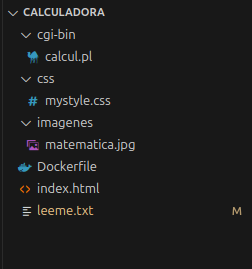
\includegraphics[width=0.5\textwidth]{lab01/latex/img/Carpetas.png}
            \end{itemize}
	
	\subsection{Creacion Html,}
	\begin{itemize}
        \item Empezamos con la creacion del html. Esto te da una idea clara de cómo se       verá la interfaz, la creacion se dara de la siguiente manera:
        \end{itemize}
	
		
	\begin{lstlisting}[language=bash,caption={Aviso que le dice al navegador que este documento es una página web en HTML5.}][H]
		<!DOCTYPE html>
	\end{lstlisting}
	\begin{lstlisting}[language=bash,caption={Etiqueta que envuelve todo el contenido de la página; indica al navegador que el idioma es español.}][H]
		<html lang="es">
	\end{lstlisting}	
	\begin{lstlisting}[language=bash,caption={Esta sección configura las bases para el funcionamiento y la presentación de la página web, asegurando que sea accesible y visualmente atractiva en diferentes dispositivos.}][H]
        <head>
            <meta charset="UTF-8">
            <meta name="viewport" content="width=device-width, initial-scale=1.0">
            <title>Lab 05 - Calculator</title>
            <link rel="stylesheet" href="css/mystyle.css">
        <head>

	\end{lstlisting}
	\begin{lstlisting}[language=bash,caption={Esta sección define el contenido visible de la página, permitiendo a los usuarios ingresar una operación matemática, enviar el formulario y ver el resultado. Está diseñada para ser facil de usar.}][H]
	      <body>
            <div class="container">
                <h1>Lab 05: Expresiones regulares en Perl</h1>
                    <form action="/cgi-bin/calcul.pl" method="get">
                        <input type="text" name="operacion" placeholder="operacion" required>
                        <br>
                        <input type="submit" value="Calculate">
                    </form>
                    <p id="result">Resultado: <span id="output"></span></p>
                </div>
         </body>
         </html>
	\end{lstlisting}
	
	\subsection{Creacion del Css} 
        \begin{lstlisting}[language=bash,caption={Esta parte del código ayuda a crear un diseño limpio y centrado en la página.}][H]
		body {
                font-family: Arial, sans-serif;
                text-align: center;
                margin: 0;
                padding: 0;
                background-image: url('../imagenes/matematica.jpg');
                background-size: cover;
                background-position: center;
                background-repeat: no-repeat;
                height: 100vh;
                display: flex;
                justify-content: center;
                align-items: center;
            }
	\end{lstlisting}
	
	\begin{lstlisting}[language=bash,caption={Este estilo ayuda a que el encabezado sea más visualmente atractivo y legible.}][H]
		h1 {
                color: #4caf50;
                text-shadow: 1px 1px 2px rgba(0, 0, 0, 0.3);
            }
	\end{lstlisting}
	\begin{lstlisting}[language=bash,caption={Establece el tamaño de la fuente y define el color del texto.}][H]
		#result {
                font-size: 1.5em;
                color: #1976d2;
            }

	\end{lstlisting}
	\begin{lstlisting}[language=bash,caption={Establece el color del texto en un rojo intenso, hace que el texto sea negrita y aumenta el tamaño de la fuente}][H]
		#output {
                color: #d32f2f;
                font-weight: bold;
                font-size: 1.8em;
            }

	\end{lstlisting}
	
	\begin{lstlisting}[language=bash,caption={Le da un estilo al contenedor principal}][H]
		.container {
                margin: 20px auto;
                padding: 30px;
                border: 1px solid #ddd;
                background-color: rgba(255, 255, 255, 0.8);
                width: 50%;
                border-radius: 10px;
                box-shadow: 0px 4px 20px rgba(0, 0, 0, 0.2);
            }
	\end{lstlisting}
	
	\begin{lstlisting}[language=bash,caption={Este estilo hace que los campos de entrada de texto sean funcionales y atractivos.}][H]
            input[type="text"] {
                width: 80%;
                padding: 12px;
                font-size: 1em;
                border: 1px solid #ccc;
                border-radius: 5px;
                transition: border 0.3s;
            }
	\end{lstlisting}
	    
	\begin{lstlisting}[language=bash,caption={Da un estilo al campo de texto cuando lo selecciona, el borde cambia a un color verde vibrante.}][H]
		input[type="text"]:focus {
                border-color: #4caf50;
            }
	\end{lstlisting}
	\begin{lstlisting}[language=bash,caption={Le dara un estilo al botón de envío}][H]
		input[type="submit"] {
                font-size: 1em;
                padding: 12px 25px;
                margin-top: 10px;
                color: #fff;
                background-color: #4caf50;
                border: none;
                border-radius: 5px;
                cursor: pointer;
                transition: background-color 0.3s;
            }
	\end{lstlisting}

        \begin{lstlisting}[language=bash,caption={Cambia el color de fondo a un verde más oscuro cuando el cursor está sobre el botón}, label={lst:color-boton}]
            input[type="submit"]:hover {
               background-color: #388e3c;
            }
        \end{lstlisting} 
        
        \begin{lstlisting}[language=bash,caption={Este le dara un estilo para el pie de página}, label={lst:color-boton}]
            footer {
                margin-top: 20px;
                font-size: 0.8em;
                color: #666;
            }
        \end{lstlisting}	
		
	\subsection{Creación del Perl}
        \begin{itemize}
            \item A continuación, se presenta un análisis detallado de cada parte del código, incluyendo la lógica utilizada para recibir, procesar y mostrar los resultados de la operación solicitada.
        \end{itemize}

        \begin{lstlisting}[language=bash,caption={Este fragmento muestra la configuración básica para iniciar el script CGI y preparar el entorno para recibir una operación desde la interfaz web.}, label={lst:color-boton}] 
            #!/usr/bin/perl
            use strict;
            use warnings;
            use CGI;
            
            my $cgi = CGI->new;
            print $cgi->header(-type => 'text/html', -charset => 'UTF-8');

            my $entrada_operacion = $cgi->param('operacion') || "";

        \end{lstlisting}	

        \begin{lstlisting}[language=bash,caption={Aquí se utiliza una expresión regular para validar y limpiar la entrada del usuario, permitiendo solo números, operadores aritméticos, paréntesis, y el operador de potencia **.}, label={lst:color-boton}]
            sub calcular_expresion {
                my ($expresion) = @_;
                $expresion =~ s/raiz\((\d+)\)/sqrt($1)/eg;
                $expresion =~ s/[^0-9+\-*\/\(\)\s\*\*]//g;
            }

        \end{lstlisting}

        \begin{lstlisting}[language=bash,caption={En esta sección divide la expresión matemática en tokens, como números y operadores, usando una expresión regular que identifica patrones específicos.}, label={lst:color-boton}]
            sub extraer_tokens {
                my ($expresion) = @_;
                my @tokens = ($expresion =~ /(\d+|\*\*|\+|\-|\*|\/|\(|\))/g);
                return @tokens;
            }

        \end{lstlisting}

        \begin{lstlisting}[language=bash,caption={Aquí se evalúan los tokens de la expresión en notación postfija, utilizando una expresión regular para identificar números, lo que permite manipular la pila y realizar las operaciones.}, label={lst:color-boton}]
            sub evaluar_postfijo {
                my @tokens = @_;
                my @pila;
            
                for my $token (@tokens) {
                    if ($token =~ /^[0-9]+$/) {
                        push @pila, $token;
                    } else {
                        my $segundo_operando = pop @pila;
                        my $primer_operando = pop @pila;
                        if ($token eq '+') {
                            push @pila, $primer_operando + $segundo_operando;
                        } elsif ($token eq '-') {
                            push @pila, $primer_operando - $segundo_operando;
                        } elsif ($token eq '*') {
                            push @pila, $primer_operando * $segundo_operando;
                        } elsif ($token eq '/') {
                            if ($segundo_operando == 0) {
                                return "No se puede dividir por cero";
                            }
                            push @pila, $primer_operando / $segundo_operando;
                        } elsif ($token eq '**') {
                            push @pila, $primer_operando ** $segundo_operando;
                        }
                    }
                }
                return pop @pila;
            }

        \end{lstlisting}

        \begin{lstlisting}[language=bash,caption={Por ultimo en este fragmento finaliza el script, generando la estructura HTML de la calculadora con el resultado. Es fundamental en CGI para mostrar el resultado de la operación ingresada.}, label={lst:color-boton}]
            print <<HTML;
            <!DOCTYPE html>
            <html lang="es">
            <head>
                <meta charset="UTF-8">
                <meta name="viewport" content="width=device-width, initial-scale=1.0">
                <title>Lab 05 - Calculator</title>
                <link rel="stylesheet" href="/css/mystyle.css">
            </head>
            <body>
                <div class="container">
                    <h1>Lab 05: Expresiones regulares en Perl</h1>
                    <form action="/cgi-bin/calcul.pl" method="get">
                        <input type="text" name="operacion" placeholder="operacion" required>
                        <br>
                        <input type="submit" value="Calcular">
                    </form>
                    <p id="result">Resultado: <span id="output">$resultado_final</span></p>
                </div>
            </body>
            </html>
            HTML

        \end{lstlisting}

    \section{Creacion del Dockerfile}
        \begin{itemize}
            \item Este archivo Dockerfile permite construir una imagen de Docker para un servidor web que soporta aplicaciones CGI en Perl. Al final, se obtiene un contenedor listo para ejecutar aplicaciones CGI en un entorno controlado y ligero, accesible a través del puerto 80.
        \end{itemize}

         \begin{lstlisting}[language=bash,caption={}, label={lst:color-boton}]
                FROM bitnami/minideb:latest

                RUN install_packages apache2 perl libapache2-mod-perl2 && \
                    install_packages libcgi-pm-perl
                
                RUN a2enmod cgi && a2enmod perl
                
                RUN sed -i '/^ScriptAlias \/cgi-bin/d' /etc/apache2/conf-enabled/serve-cgi-bin.conf && \
                    echo "ScriptAlias /cgi-bin/ /usr/lib/cgi-bin/" >> /etc/apache2/conf-enabled/serve-cgi-bin.conf && \
                    echo "<Directory \"/usr/lib/cgi-bin\">\n    AllowOverride None\n    Options +ExecCGI\n    Require all granted\n</Directory>" >> /etc/apache2/conf-enabled/serve-cgi-bin.conf
                
                RUN echo "ServerName localhost" >> /etc/apache2/apache2.conf
                
                COPY index.html /var/www/html/
                COPY css /var/www/html/css
                COPY imagenes /var/www/html/imagenes
                
                COPY cgi-bin/calcul.pl /usr/lib/cgi-bin/
                RUN chmod +x /usr/lib/cgi-bin/calcul.pl
                
                EXPOSE 80
                
                CMD ["apachectl", "-D", "FOREGROUND"]

         \end{lstlisting}
    
        \section{Prueba de la correcta operacion de la Calculadora}
            \begin{itemize}
                \centering
                \item [] 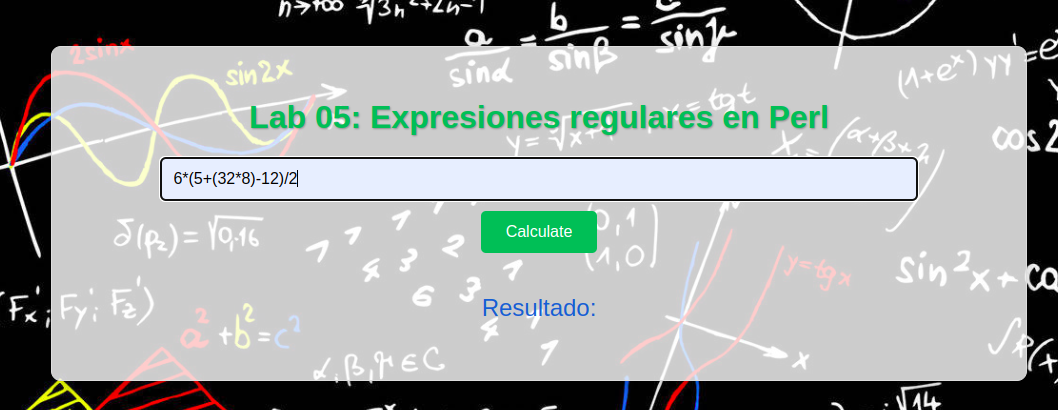
\includegraphics[width=1 \textwidth]{Lab5/latex/img/Pruebas/prueba1.png}
                \item [] 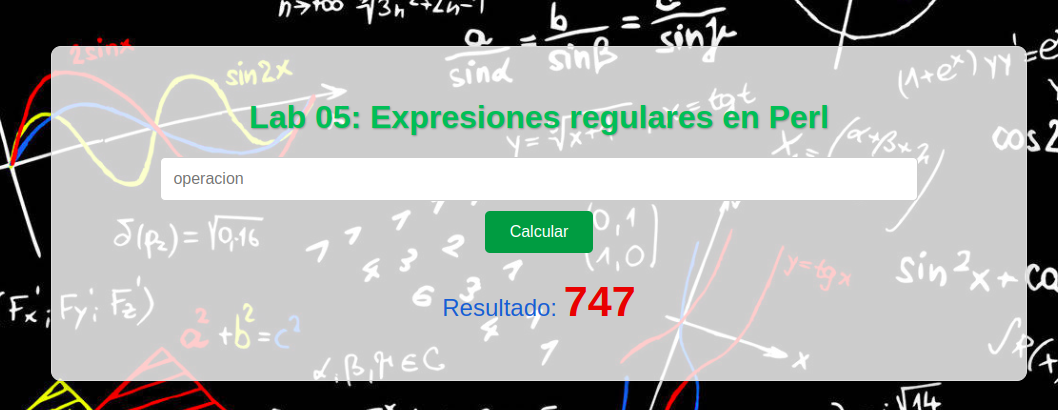
\includegraphics[width=1 \textwidth]{Lab5/latex/img/Pruebas/rptaPrueba1.png}
                \item [] 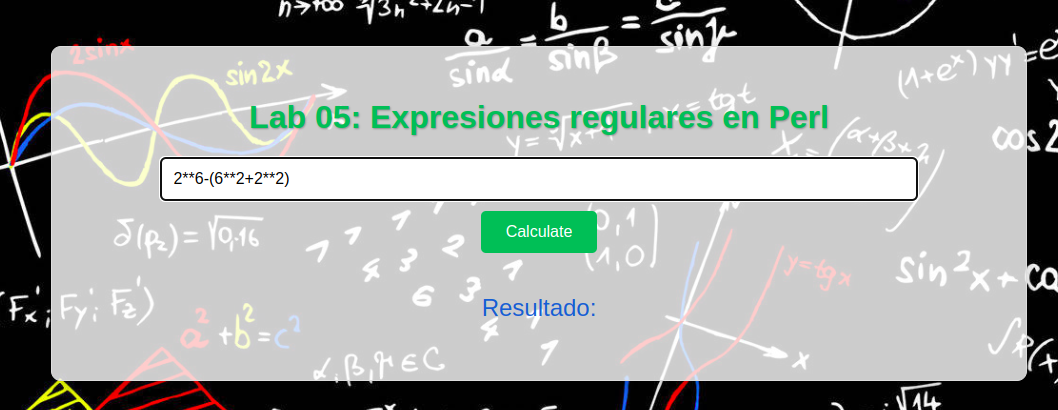
\includegraphics[width=1 \textwidth]{Lab5/latex/img/Pruebas/prueba2.png}
                \item [] 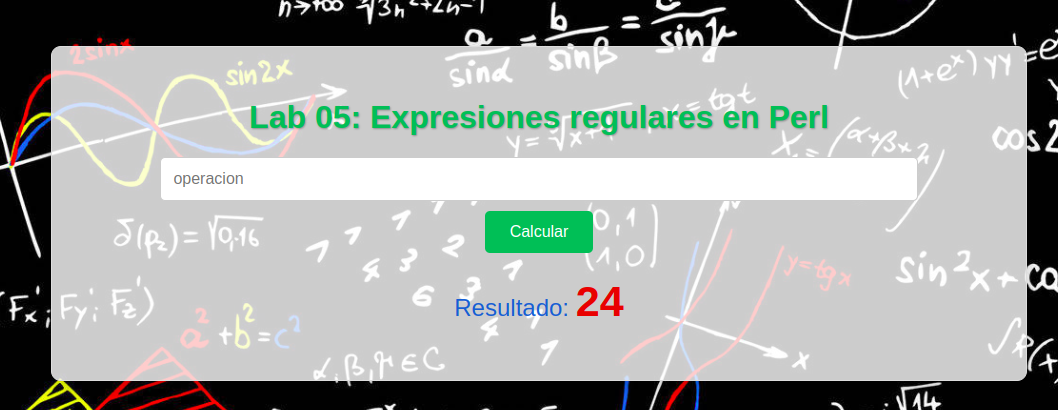
\includegraphics[width=0.9 \textwidth]{Lab5/latex/img/Pruebas/rptaPrueba2.png}
                \item [] 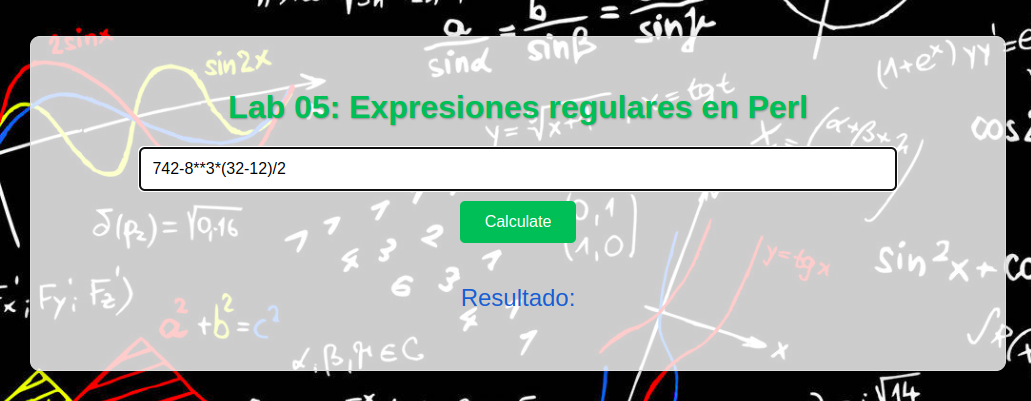
\includegraphics[width=0.9 \textwidth]{Lab5/latex/img/Pruebas/prueba3.png}
                \item [] 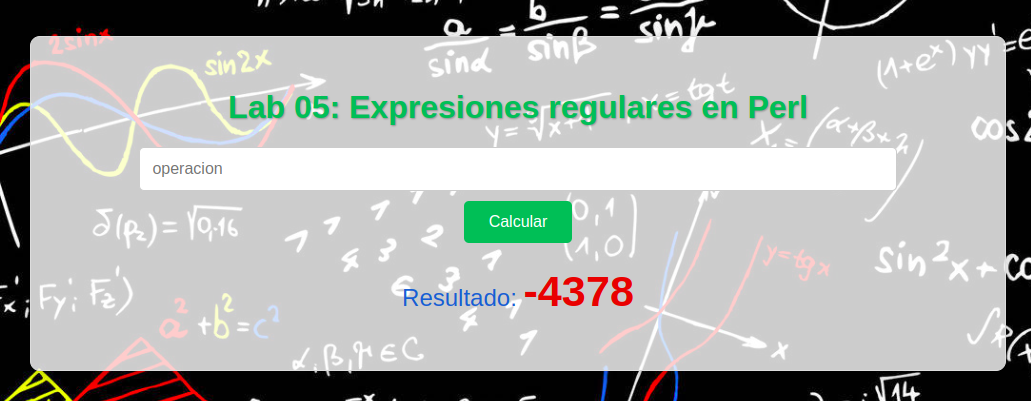
\includegraphics[width=0.9 \textwidth]{Lab5/latex/img/Pruebas/rptaPrueba3.png}
                
            \end{itemize}
   		

	\section{\textcolor{red}{Rúbricas}}
	
	\subsection{\textcolor{red}{Entregable Informe}}
	\begin{table}[H]
		\caption{Tipo de Informe}
		\setlength{\tabcolsep}{0.5em} % for the horizontal padding
		{\renewcommand{\arraystretch}{1.5}% for the vertical padding
		\begin{tabular}{|p{3cm}|p{12cm}|}
			\hline
			\multicolumn{2}{|c|}{\textbf{\textcolor{red}{Informe}}}  \\
			\hline 
			\textbf{\textcolor{red}{Latex}} & \textcolor{blue}{El informe está en formato PDF desde Latex.}   \\ 
			\hline 
						
		\end{tabular}
	}
	\end{table}
	
	\clearpage
	
	\subsection{\textcolor{red}{Rúbrica para el contenido del Informe y demostración}}
	\begin{itemize}			

		\item El alumno debe autocalificarse en la columna \textbf{Estudiante} de acuerdo a la siguiente tabla:
	
	\end{itemize}
		
           \begin{center}
        \begin{table}[h!]
        \renewcommand{\arraystretch}{2}
        \begin{tabular}{|>{\centering\arraybackslash}m{3cm}|>{\arraybackslash}m{7cm}|>{\centering\arraybackslash}m{1cm}|>{\centering\arraybackslash}m{2cm}|>{\centering\arraybackslash}m{1cm}|}
        \hline
        \rowcolor[HTML]{D9EAD3} 
        \textbf{ÍTEM}      & \textbf{DESCRIPCIÓN} & \textbf{EXC.} & \textbf{PROCESO} & \textbf{DEF.} \\ \hline
        Código fuente      & Hay porciones de código fuente importantes con numeración y explicaciones detalladas de sus funciones. & 4 &  & \\ \hline
        Ejecución          & Se incluyen ejecuciones/pruebas del código fuente explicadas gradualmente hasta llegar al código final del requerimiento del laboratorio. & 4 &  &  \\ \hline
        Pregunta           & Se responde con completitud a la pregunta formulada en la tarea. (El profesor puede preguntar para refrendar calificación). Si no se le entregó pregunta, usted recopile información relevante para el laboratorio desde diferentes medios, referenciándola correctamente (máximo 2 caras). &  & 2 &  \\ \hline
        Ortografía         & El documento no muestra errores ortográficos. &  & 2 &  \\ \hline
        Madurez            & El informe muestra de manera general una evolución de la madurez del código fuente, explicaciones puntuales pero precisas y un acabado impecable. (El profesor puede preguntar para refrendar calificación). &  & 2 &  \\ \hline
        \rowcolor[HTML]{F4CCCC} 
        \textbf{CALIFICACIÓN} & & \textbf{8} & \textbf{6} & \textbf{} \\ \hline
        \end{tabular}
        \end{table}
        \end{center}

       \vspace{0.3cm}
    
            \textbf{\Large CALIFICACIÓN TOTAL: \textcolor{red}{14}} 
        
        \section{Referencias}
        \begin{itemize}			
        	\item \url{https://carontestudio.com/blog/como-poner-una-imagen-de-fondo-en-html/}
        	\item \url{https://metacpan.org/dist/POD2-ES/view/lib/POD2/ES/perlop.pod}
        \end{itemize}	
     \end{document}
